% Required packages: amsmath, pgfplots
% Required TikZ libraries: none
% Target width: 155 mm maximum
% Minimum text size: 9 pt
% Colour/greyscale intent: colour and greyscale, redundant line styles and direct labels
% Generated by calculate_sufficiency.py from decision-sufficiency.inputs.json.
% All values are illustrative; conditional intervals are not confidence intervals.
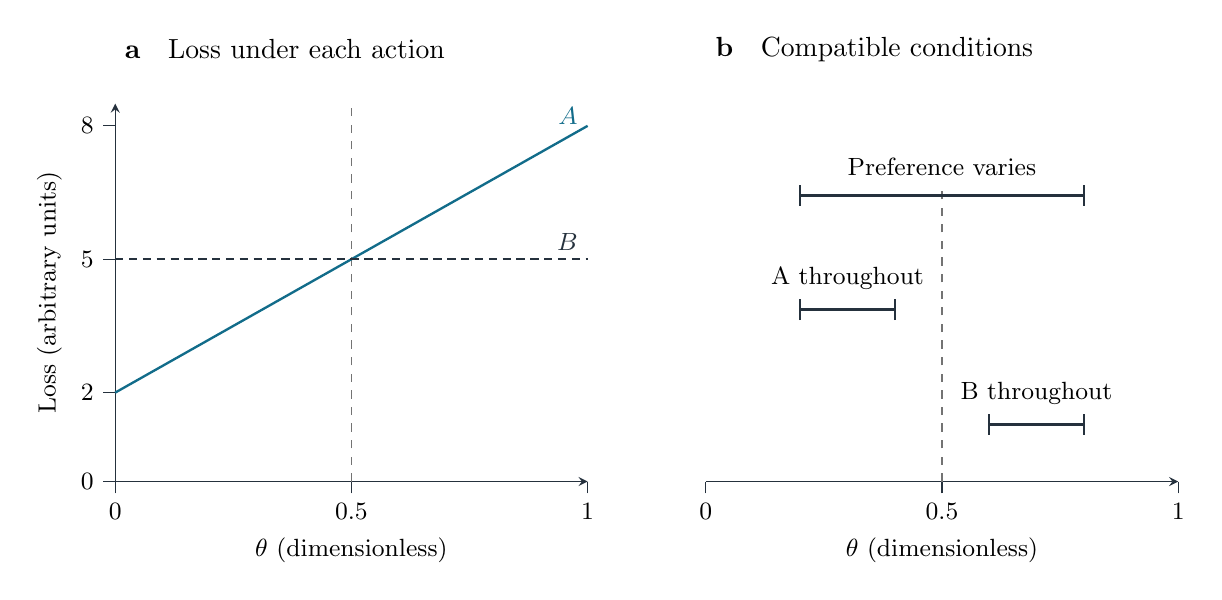
\begin{tikzpicture}[font=\fontsize{9}{11}\selectfont]
\definecolor{ink}{HTML}{25313D}
\definecolor{accent}{HTML}{126C8A}
\pgfplotsset{compat=1.18,
  decision axis/.style={
    width=60mm, height=48mm, scale only axis,
    xmin=0, xmax=1, xtick={0,0.5,1},
    axis lines=left, axis line style={line width=0.45pt, draw=ink},
    tick style={line width=0.45pt, draw=ink},
    tick align=outside, ticklabel style={font=\fontsize{9}{11}\selectfont},
    xlabel={$\theta$ (dimensionless)},
    xlabel style={font=\fontsize{9}{11}\selectfont},
    every axis plot/.append style={no marks},
    clip=false, enlargelimits=false}}
\begin{axis}[decision axis, name=losses, at={(0mm,0mm)}, anchor=south west,
  ymin=0, ymax=8.5, ytick={0,2,5,8},
  ylabel={Loss (arbitrary units)},
  ylabel style={font=\fontsize{9}{11}\selectfont},
  title={\textbf{a}\quad Loss under each action},
  title style={font=\fontsize{10}{12}\selectfont, at={(0,1.10)}, anchor=west}]
\addplot[draw=black!55, dashed, line width=0.45pt] coordinates {(0.5,0) (0.5,8.5)};
\addplot[draw=accent, line width=0.85pt] coordinates {(0.0,2.0) (1.0,8.0)};
\addplot[draw=ink, densely dashed, line width=0.85pt] coordinates {(0.0,5.0) (1.0,5.0)};
\node[anchor=south east, text=accent, inner sep=0pt] at (axis cs:0.98,8.02) {$A$};
\node[anchor=south east, text=ink, inner sep=0pt] at (axis cs:0.98,5.18) {$B$};
\end{axis}
\begin{axis}[decision axis, at={(75mm,0mm)}, anchor=south west,
  ymin=0.5, ymax=3.8, ytick=\empty, axis y line=none,
  title={\textbf{b}\quad Compatible conditions},
  title style={font=\fontsize{10}{12}\selectfont, at={(0,1.10)}, anchor=west}]
\addplot[draw=black!55, dashed, line width=0.45pt] coordinates {(0.5,0.5) (0.5,3.1)};
\addplot[draw=ink, line width=1.1pt] coordinates {(0.2,3) (0.8,3)};
\addplot[draw=ink, line width=0.6pt] coordinates {(0.2,2.91) (0.2,3.09)};
\addplot[draw=ink, line width=0.6pt] coordinates {(0.8,2.91) (0.8,3.09)};
\node[anchor=south, inner sep=0pt] at (axis cs:0.5,3.17) {Preference varies};
\addplot[draw=ink, line width=1.1pt] coordinates {(0.2,2) (0.4,2)};
\addplot[draw=ink, line width=0.6pt] coordinates {(0.2,1.91) (0.2,2.09)};
\addplot[draw=ink, line width=0.6pt] coordinates {(0.4,1.91) (0.4,2.09)};
\node[anchor=south, inner sep=0pt] at (axis cs:0.3,2.17) {A throughout};
\addplot[draw=ink, line width=1.1pt] coordinates {(0.6,1) (0.8,1)};
\addplot[draw=ink, line width=0.6pt] coordinates {(0.6,0.91) (0.6,1.09)};
\addplot[draw=ink, line width=0.6pt] coordinates {(0.8,0.91) (0.8,1.09)};
\node[anchor=south, inner sep=0pt] at (axis cs:0.7,1.17) {B throughout};
\end{axis}
\end{tikzpicture}
